%%%%%%%%%%%%%%%%%%%%%%%%%%%%%%%%%%%%%%
% START ADDING TEXT HERE
%
% Feel free to use \include commands to structure text in smaller
% pieces
%
%%%%%%%%%%%%%%%%%%%%%%%%%%%%%%%%%%%%%%


% Abstract gives a brief summary of the main points of a paper:
\begin{abstract}
\textbf{Abstract - Internet of Things (IoT) is emerging rapidly in recent years, IoT applications are producing huge amount of heterogeneous data. This can lead to disaster as IoT applications have minimum computation power. Fog Computing resolves this issue by providing not only computational resources but also proper management and Orchestration for these IoT applications. But providing proper resource scheduling for these applications is still a challenge in Fog Computing. This seminar paper discusses the solution available for proper scheduling of applications based on network resources such as latency, bandwidth, etc. Kubernetes is used as Fog Computing infrastructure and applications are deployed as \emph{pod} (set of containers). Default Kubernetes scheduler only considered the computational resources and does not consider the network resources which is important in the case of data-sensitive applications. Results show that network-based resource provisioning performs better than the default scheduling technique. Detail comparison is provided between using network-based resource provisioning and other available solutions in the market.}
\end{abstract}

% the actual content, usually separated over a number of sections
% each section is assigned a label, in order to be able to put a
% crossreference to it

\section{Introduction}
\label{sec:introduction}
\begin{figure}
  \centering
  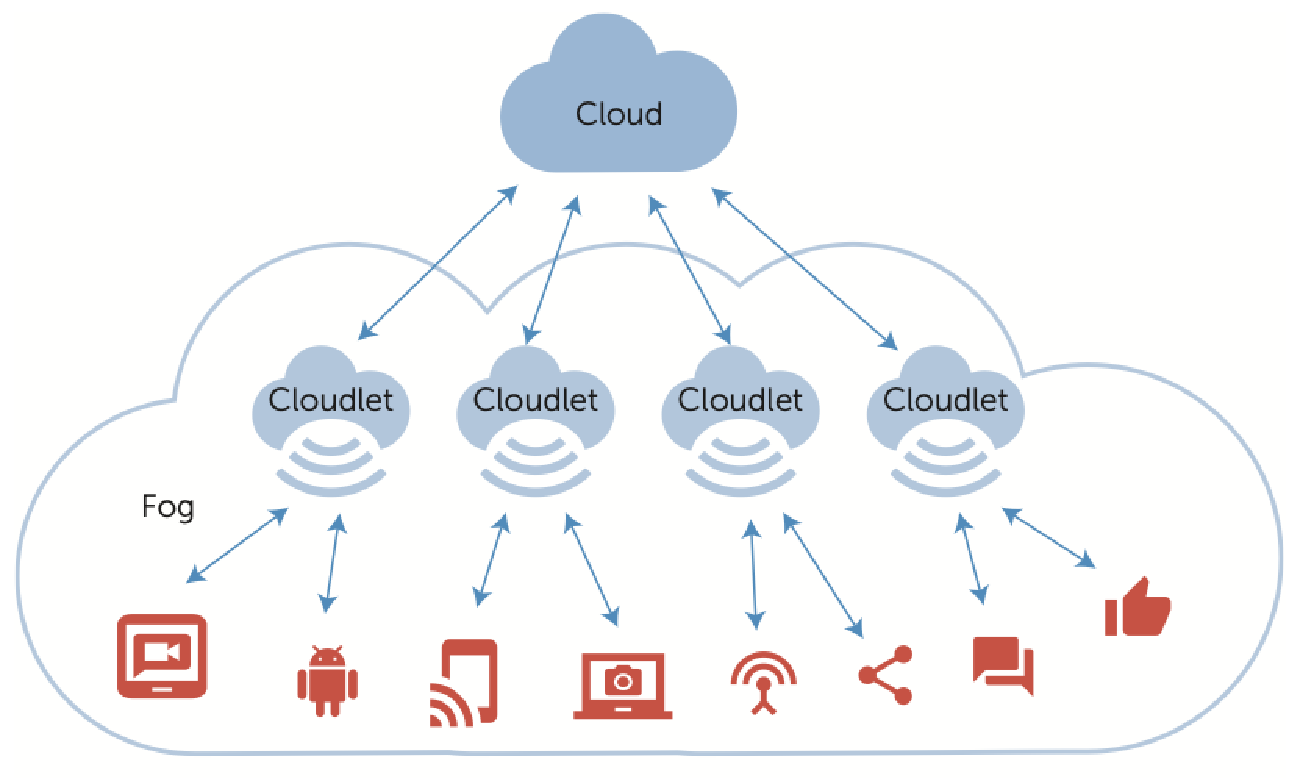
\includegraphics[width=70mm]{figures/mlcn-fog-1.pdf}
  \caption{Fog computing: Top-level overview\cite{Bittencourt2017}}
  \label{fig:fog-arch}
\end{figure}
In recent years with the evolution of technology, the Internet of Things (IoT) devices are increasing day by day. According to Ericsson mobility report\cite{}, there will be a 17\% (approx. 22.3 billion) increase in IoT devices by 2024. Functionally IoT is defined as \emph{"The Internet of Things allows people and things to be connected Anytime, Anyplace, with Anything and Anyone"} \cite{European commission 2008}. IoT devices have served mankind in many ways such as from smart houses to smart cities, smart transportation systems, and many medical applications. These IoT applications enable many devices connected to the network and generate a lot of heterogeneous data also known as BigData which requires special data processing models and Infrastructure support. Processing BigData required a lot of resources and cloud computing theoretically provides it unlimited resources\cite{fog-comp-survey}. But there is a downside of using cloud computing for such complex computation as it is more costly when it comes to computation power, storage, and bandwidth. Computation needs to be performed at the node level and only the aggregated data need to send to the central node for further computations and analysis. This de-centralized approach will save a lot of computation power as well as bandwidth requriments\cite{fog-comp-survey}. To overcome the downside of cloud computing, the terminology fog computing is used. Fog computing allows the computation at the edge of the network instead of central core. \par
Fog computing is defined as \emph{"An architecture that uses one or a collaborative multitude of end-user clients or near-user edge devices to carry out a substantial amount of storage (rather than stored primarily in cloud data centers), communication (rather than routed over the internet backbone), and control, configuration, measurement and management (rather than controlled primarily by network gateways such as those in the LTE (telecommunication) core)”}\cite{Chiang 2015; Aazam and Huh 2014}. Traditionally, user applications running in the cloud access the cloud core network through access points for data exchange to fetch data from data-centers \cite{Bittencourt2017}. In fog computing these access points also serves as resource providers such as computation power and storage etc. and are called "cloudlets"\cite{Bittencourt2017}. Figure \ref{fig:fog-arch} show the top-level architecture of the fog computing. \par
Fog computing is responsible for providing resources to IoT devices for processing. Traditionally these resources are allocated as VMs from different cloud infrastructures such as AWS, Google, OpenStack, etc. to run the applications. VMs are considered resource greedy and require more computational resources. An alternate is to use the Containers such as Docker which is light-weight, requires fewer resources and based on micro-service architecture. Large applications are split into containers based on the main processes of the application. This increasing number of containers per application required the proper monitoring for health check and resource consumption. The most commonly used orchestrator for containers is Kubernetes. \par
Kubernetes act as IaaS for fog computing to provide resources for IoT applications. Kubernetes is an open-source platform for management, deployment, and scaling of containers. In Kubernetes, applications are deployed as pod consisting of multiple containers. When the configuration of the deploying application is passed to Kubernetes, it checks for the availability of resources and deploys afterward. Kubernetes default resource scheduler monitors and deploys the pod using computation power-based scheduling mechanism and does not consider latency and available bandwidth, which is considered important while dealing with the data-centric application. An example of a data-centric application is a weather forecast that receives data from scattered IoT devices and provide prediction. If the data is lost or delayed due to higher latency and poor bandwidth, timely decisions cannot be made that lead to disaster. To overcome this drawback of Kubernetes, the author proposed an alternate Kubernetes scheduler that considers network resources along with computational resources.
\section{Background}
\label{sec:backgroud}
This section explains about the Kubernetes main components, working as Orchestrator and built-in resource provisioning techniques.
\subsection{Kubernetes Main Components}
\label{sec:k8s_main_comp}

\begin{figure}
  \centering
  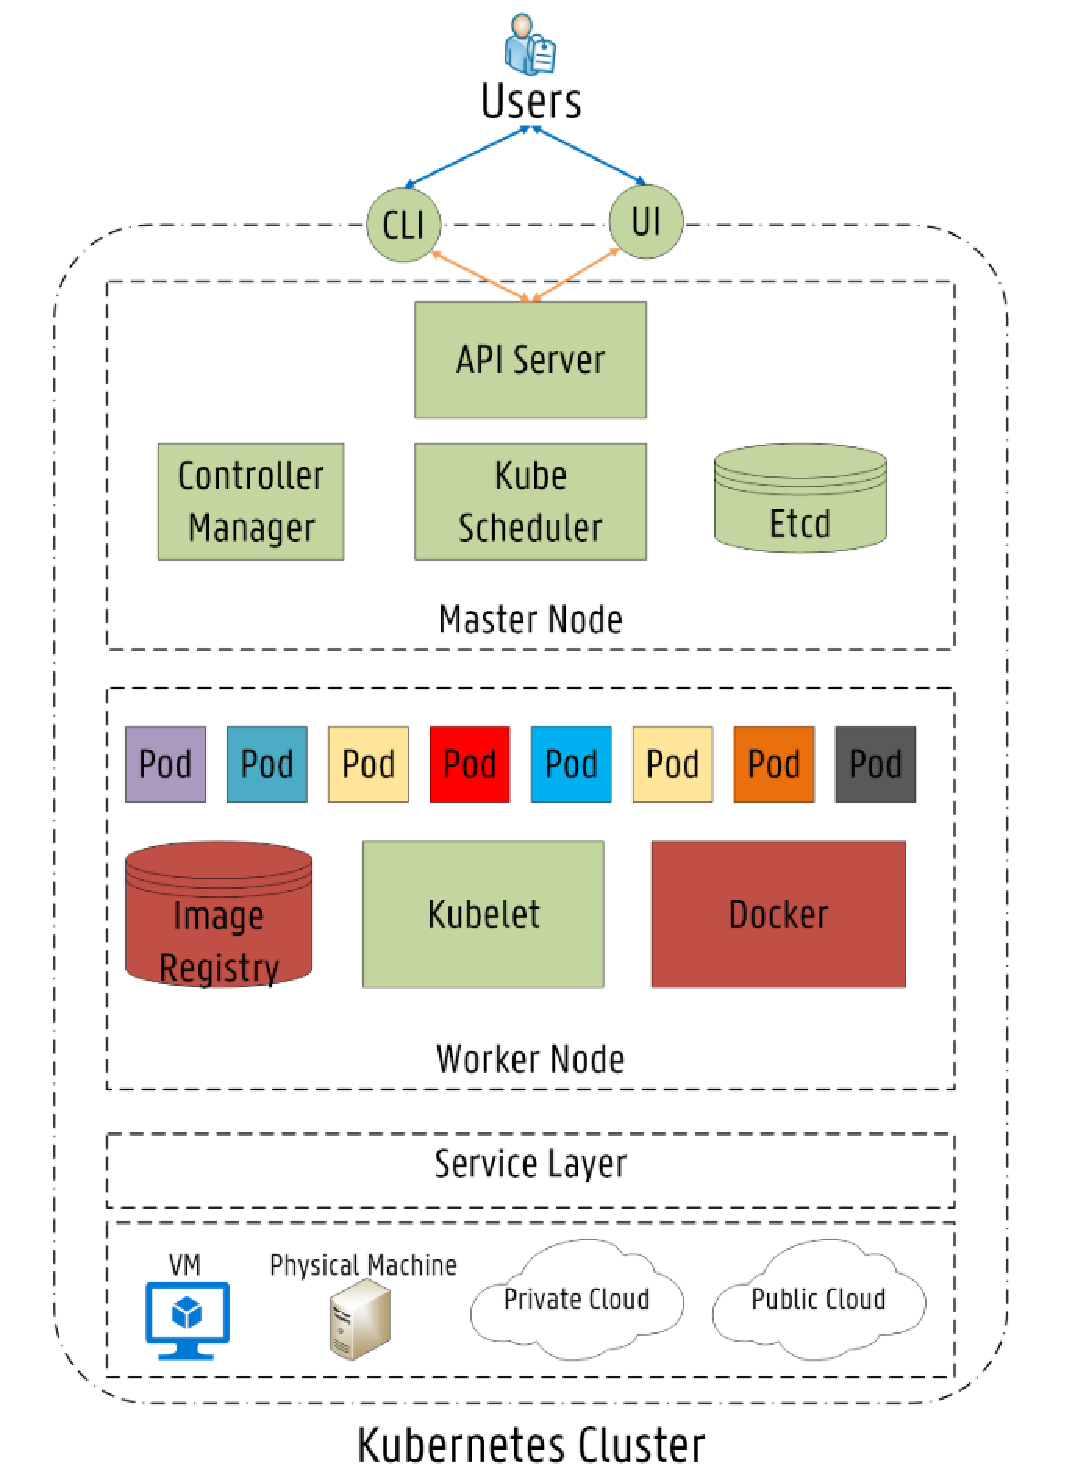
\includegraphics[width=68mm]{figures/mlcn-k8s-components.pdf}
  \caption{Kubernetes Cluster: Main Components\cite{Santos2019}}
  \label{fig:k8s-comp}
\end{figure}
Kubernetes is an open-source project that manages the container-based applications deployed over multiple hosts. Kubernetes act as Orchestrator which is responsible for deploying, managing, scaling of container-based application\cite{kubernetes-github-repo}. Figure \ref{fig:k8s-comp} shows the main components coupled to work as one unit called kubernetes. It is based on master-slave model, consisting of one \emph{master node} and multiple \emph{worker nodes} \cite{Santos2019}. \emph{worker nodes} can be either physical or virtual resources such as physical servers or virtual machines. \emph{master node} communicates with \emph{worker nodes} using \emph{API} calls. \emph{API server} uses RESTFul API, for managing all the \emph{API} calls is also part of \emph{master node}. End-users communicate with the Kubernetes cluster using \emph{Kubectl}, which forward user requests to \emph{API server} and intern gets the result. \emph{Etcd} stores the data as key-value pair, which is used to store all configurations, states. It is one of the main components of Kubernetes, which maintains the state across the cluster for synchronization of data. \emph{Control Manager} is responsible for monitoring of \emph{Etcd}. For any state change of cluster, \emph{Control Manager} forwards the new state request using \emph{API server}. \emph{Kube Scheduler} is discussed later in section \ref{sec:k8s_scheduler}. On \emph{worker node}, node agent known as \emph{Kubelet} which is responsible for maintain state-based on \emph{API server} request. For any state change communicated by \emph{API server}, \emph{Kubelet} performs the desired operation such as starting or deleting of Docker containers. \emph{Image Registry} is responsible for managing the images required to create the container applications. \emph{Pod} is the main component of \emph{worker node} where all the applications are deployed. Single \emph{Pod} represents the application that consists of multiple containers based on the services of the application. \emph{Pod} is the collections of containers, volumes in an isolated environment which means there is no cross-communication between two \emph{Pods}. Containers running in a \emph{Pod} share the same IP Address \cite{Santos2019}. Containers communicate using different ports, hence there is a limitation to this approach as two containers listening on same port cannot be in same \emph{Pod}\cite{Santos2019}.
\subsection{Kubernetes as Orchestrator}
\label{sec:k8s_orchestrator}
Orchestrator is responsible for automating the processes that require a lot of human effort. As discussed in \cite{containerjournal}, Orchestrator is responsible for the following:
\begin{itemize}
  \item Starting or stopping of different applications.
  \item Ensure the Scalability of application for high usage demands.
  \item Management of load across different nodes to avoid resource overhead.
  \item Monitoring the health of applications.
\end{itemize}
There are many Orchestrator currently available, but the most widely used are OpenStack and Kubernetes.
\begin{enumerate}
  \item \textbf{OpenStack Orchestration:} It provides template-based orcestration for cloud application to run on OpenStack. Template allows to create resources such as Virtual machines(Instances), Storage (Volumes), Networks etc. These resources are coupled together as OpenStack \emph{Project} to run cloud application\cite{openstackOrchestrator}.
  \item \textbf{Kubernetes Orchestration:} It is responsible for automating deployment, scaling, and management of container-based applications. \emph{master node} orchestrates the application across various \emph{worker node} based on resource availability.
\end{enumerate}
\subsection{Kubernetes Resource Provisioning}
\label{sec:k8s_scheduler}
\begin{figure}
  \centering
  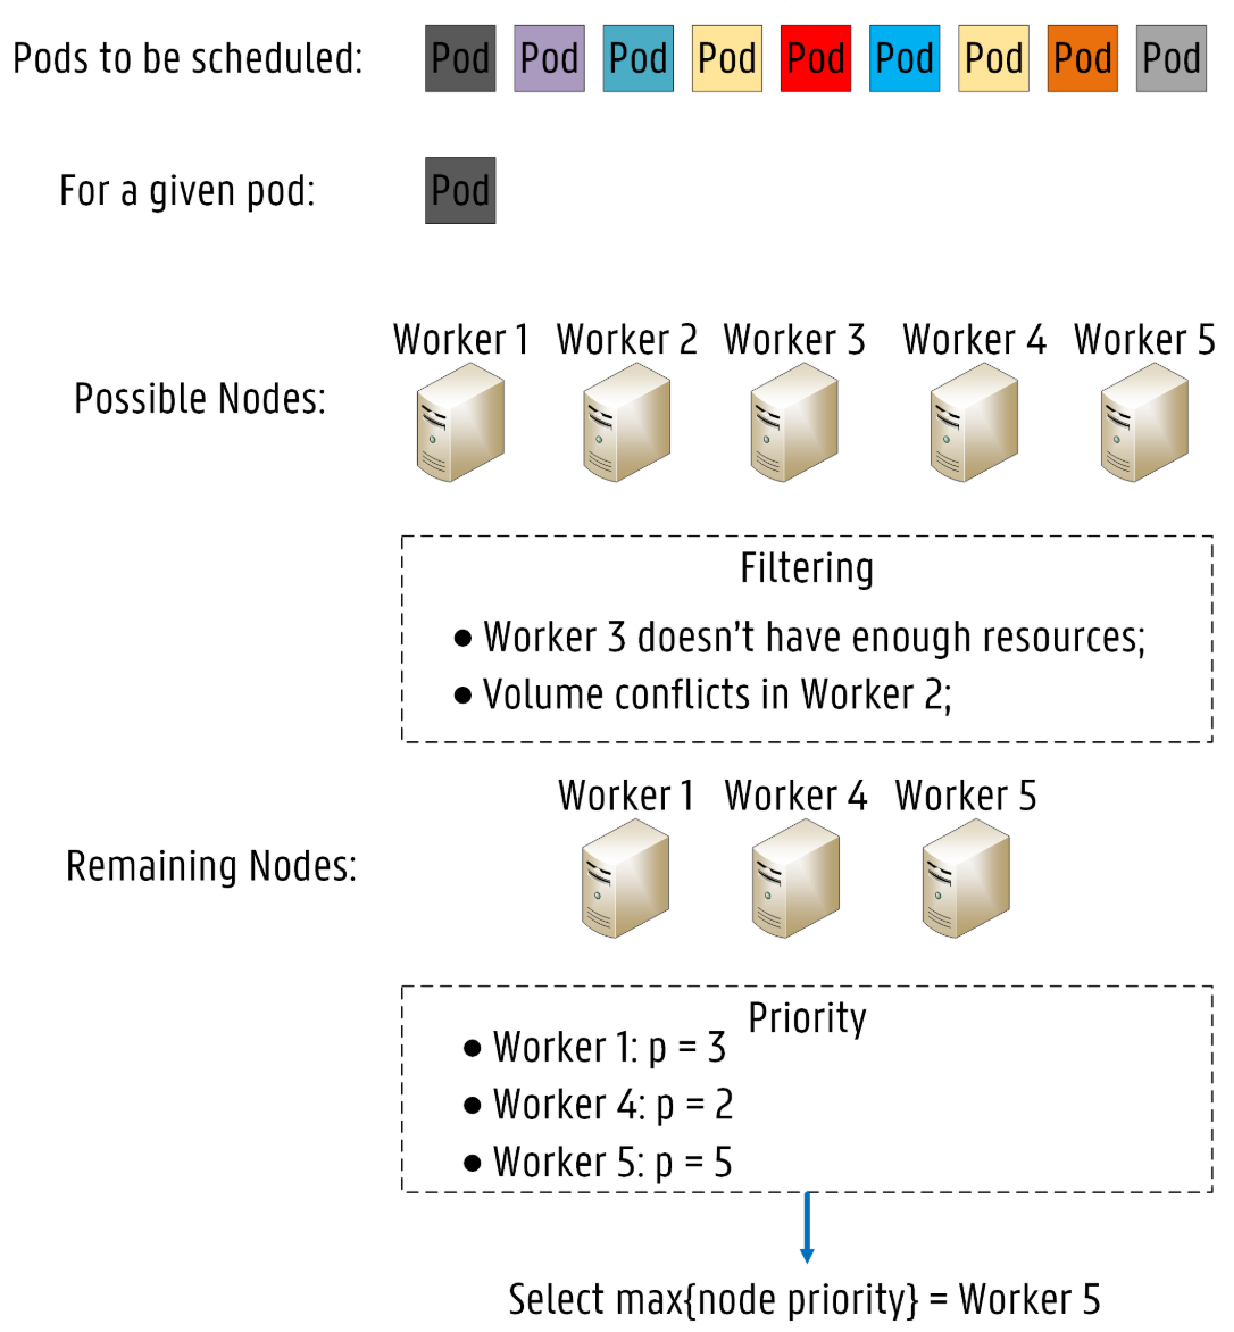
\includegraphics[width=\linewidth]{figures/mlcn-k8s-scheduler.pdf}
  \caption{Kubernetes Scheduler: Working\cite{Santos2019}}
  \label{fig:k8s-sch}
\end{figure}
When the user provides the configuration for creating new \emph{pod} using \emph{Kubectl}. The \emph{Pod} is added to the waiting queue with all the other \emph{pods}. \emph{Kube-Scheduler} which is the default scheduler of Kubernetes, decides which \emph{pod} deploys on which \emph{worker node} based on some criteria. Figure \ref{fig:k8s-sch} shows the default scheduling mechanism where the \emph{pod} is deployed by passing through following steps: \emph{node filtering} and \emph{node priority or scoring}\cite{Santos2019}. In the kubernetes cluster, \emph{worker nods} meeting the requirement of \emph{ped} are called \emph{feasible nodes}\cite{k8s}.
\subsubsection{\emph{Node Filtering}}
\label{sec:node-filter}
The first step of deploying \emph{pod} is \emph{node filtering} in which \emph{Kube-Scheduler} will select the \emph{feasible nodes} based on the \emph{pod} configuration by applying some filters. These filters are also called \emph{predicates}. Following is the list of \emph{predicates} that are supported by \emph{Kube-Scheduler}\cite{k8s}:
\begin{enumerate}
  \item \textbf{PodFitsHostPorts:} This filter checks the \emph{worker node} for the ports requested by the \emph{pod}.
  \item \textbf{PodFitHost:} This filter checks for \emph{worker node} with hostname mentioned in a \emph{pod} configuration.
  \item \textbf{PodFitsResources:} This filter checks for the available resources i.e. CPUs and Memory to run the \emph{pod}.
  \item \textbf{NoDiskConflict:} This filter checks the \emph{worker node} for the volumes requested by the \emph{pod} and is already mounted.
  \item \textbf{CheckNodeMemoryPressure:} This filter checks the \emph{worker node} for the over-utilization of Memory.
  \item \textbf{CheckNodeDiskPressure:} This filter checks the \emph{worker node} disk space and filesystem, sufficient to run the \emph{pod}.
  \item \textbf{CheckNodeCondition:} This filter checks the \emph{worker node} for available disk space, networking configuration and that of \emph{Kubelet} is reachable or not.
  \item \textbf{PodMatchNodeSelector:} This filter search for the \emph{worker node} based on the label mentioned in \emph{pod} configuration. These labels allow the user to deploy the \emph{pod} on specific \emph{worker node}(node-affinity)\cite{Santos2019}. Another use case of using a label is to restrict the \emph{pod} deployment based on other \emph{pod} already deployed on that \emph{worker node} (pod-anti-affinity) \cite{Santos2019}. These affinity rules are based on \emph{Tolerations} and \emph{Taints} which are defined as key-value pairs along with their effects. \emph{Tolerations} are defined in \emph{pod} configration whereas \emph{Taints} are set for \emph{worker node}. Both \emph{Tolerations} and \emph{Taints} work together to ensure \emph{pod} is not deployed on inappropriate \emph{worker node} \cite{k8s}.
\end{enumerate}
Using the above-mentioned filters(\emph{predicates}), \emph{Kube-Scheduler} returns the \emph{feasible node} for \emph{pod} deployment. If no \emph{feasible node} is found, \emph{pod} remains unscheduled and error message is generated for failed deployment \cite{Santos2019}. If the list of the \emph{feasible nodes} is returned as the result of applying filters then \emph{Kube-Scheduler} moves to second step \emph{node priority or scoring}.
\subsubsection{\emph{Node Priority/Scoring}}
\label{sec:node-priority}
\emph{Kube-Scheduler} assigns a rank to each \emph{worker node} that passes the \emph{node filtering} stage. These ranks/priorities sort the list of \emph{worker nodes} based on best-fit for \emph{pod} deployment. These priorities are set based on the following criteria\cite{k8s}:
\begin{enumerate}
  \item \textbf{SelectorSpreadPriority:} "This priority algorithm tries to minimize the number of deployed pods belonging to the same service on the same node or on the same zone/rack"\cite{Santos2019}.
  \item \textbf{InterPodAffinityPriority:} This priority sets the score for \emph{worker node} based on the pod-affinity rule mentioned above.
  \item \textbf{LeastRequestedPriority:} This priority sets the score for \emph{worker node} based on the higher available resources i.e. CPU and Memory.
  \item \textbf{MostRequestedPriority:} This priority sets the score for \emph{worker node} based on the minimum resource requirement for \emph{pod} deployment.
  \item \textbf{RequestedToCapacityRatioPriority:} This priority sets the score for \emph{worker node} based on a request to capacity using ResourceAllocationPriority.
  \item \textbf{BalancedResourceAllocation:} This priority selects the \emph{worker node} with balanced resource utilization.
  \item \textbf{NodeAffinityPriority:} This priority selects the \emph{worker node} based on the node-affinity rule. \emph{Worker node} with the required label will be given priority.
  \item \textbf{TaintTolerationPriority:} This priority sets the score for \emph{worker node} based on their \emph{taints} with respect to \emph{tolerations} mentioned in \emph{pod} configuration\cite{Santos2019}.
  \item \textbf{ImageLocalityPriority:} This priority sets the score for the \emph{worker node} based on the availability of the image on \emph{worker node} required to build the containers for a \emph{pod}.
  \item \textbf{EqualPriority:} This priority sets equal weight to all the \emph{worker nodes}.
\end{enumerate}
\begin{figure*}
  \centering
  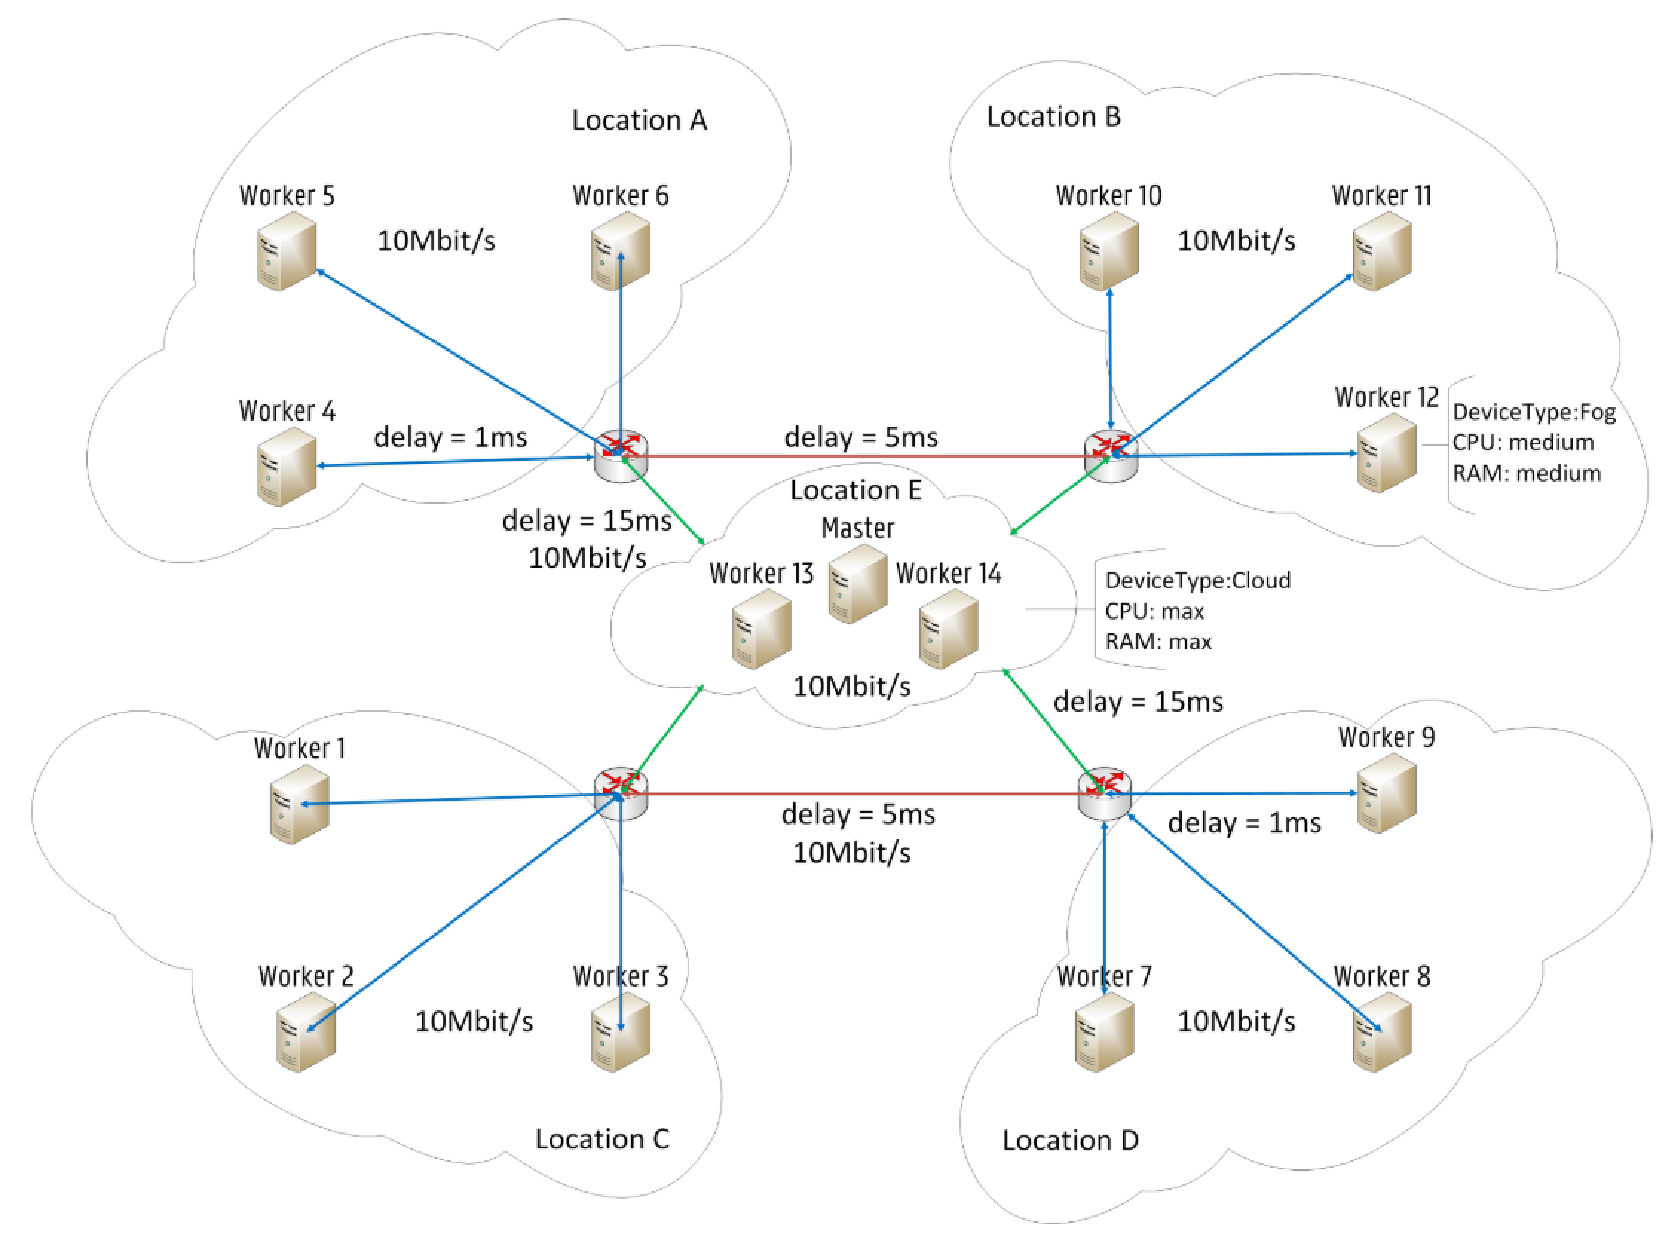
\includegraphics[width=80mm]{figures/mlcn-fog-k8s-infra.pdf}
  \caption{Kubernetes-based Fog Computing Infrastructure\cite{Santos2019}}
  \label{fig:fog-k8s-infra}
\end{figure*}
\section{Kubernetes Network-based Resource Provisioning}
\label{sec:k8s_ns}
The default \emph{Kube-Scheduler} works efficiently for resources such as CPU, Memory, and storage but does not consider the networking resource which is considered a critical resource in many use-case scenarios. Considering one application of Fog Computing such as IoT based smart cities which is a data-sensitive use case. Ensuring that no data is lost, networking resources need to be configured properly\cite{Santos2019}. Default \emph{Kube-Scheduler} does not check the network latency and available bandwidth for the \emph{worker node}. In order to cater to this drawback, the author in \cite{Santos2019} proposed a scheduler that checks for the network resources along with the default \emph{Kube-Scheduler}. \par
Kubernetes allows three ways to extend the \emph{Kube-Scheduler} to allow the network-based resource provisioning\cite{k8s}.
\begin{itemize}
  \item Extending \emph{Kube-Scheduler} by adding new \emph{filter/predicates} or \emph{priority/scoring}.
  \item Build the new scheduler that replaces the default \emph{Kube-Scheduler} or two schedulers work together.
  \item Define the scheduling process that can be called by the default \emph{Kube-Scheduler} before scheduling the resources.
\end{itemize}
As per \cite{Santos2019}, the author used the third approach that allows the default \emph{Kube-Scheduler} to apply \emph{filters} and calculate the \emph{priority} of the \emph{worker nodes} afterward the external scheduling process function is called. When the scheduling process is called, two function calls are generated\cite{Santos2019}, first one for the list of \emph{worker nodes} as the result of \emph{filtering/predicates} of \emph{Kube-Scheduler}\cite{Santos2019}. Second, for the list of \emph{worker nodes} after calculating the \emph{priority} using \emph{Kube-Scheduler}\cite{Santos2019}. For Kubernetes to work as Fog Computing infrastructure, "affinity/anit-affinity" rules and node labeling is used as shown in figure \ref{fig:fog-k8s-infra}. The infrastructure consists of 1 \emph{master node} and 14 \emph{worker nodes}. All nodes are labeled with \{\emph{Min, High, Medium}\} for resources such as \{\emph{CPU, Memory}\}\cite{Santos2019}. These nodes are further labeled by \{\emph{DeviceType}\} based on their functionality and geographical positioning by \emph{tains} such as \{\emph{Cloud, Fog}\}\cite{Santos2019}. These rules and node labeling will help inefficient deployment of \emph{pods} on certain \emph{worker nodes}. Considering the delay-sensitive application scenario, the data collecting node which is near to data processing node is taken into account due to time dependency\cite{Santos2019}. For improving \emph{pod} deployment based on the above scenario, all \emph{worker nodes} are further labeled for Round Trip Time(RTT) from the \emph{master node} as shown in figure\ref{fig:k8s-rtt}.\par
The external scheduling process further calls two schedulers and these schedulers will filter out \emph{worker  nodes} based on networking resources.
\begin{figure}
  \centering
  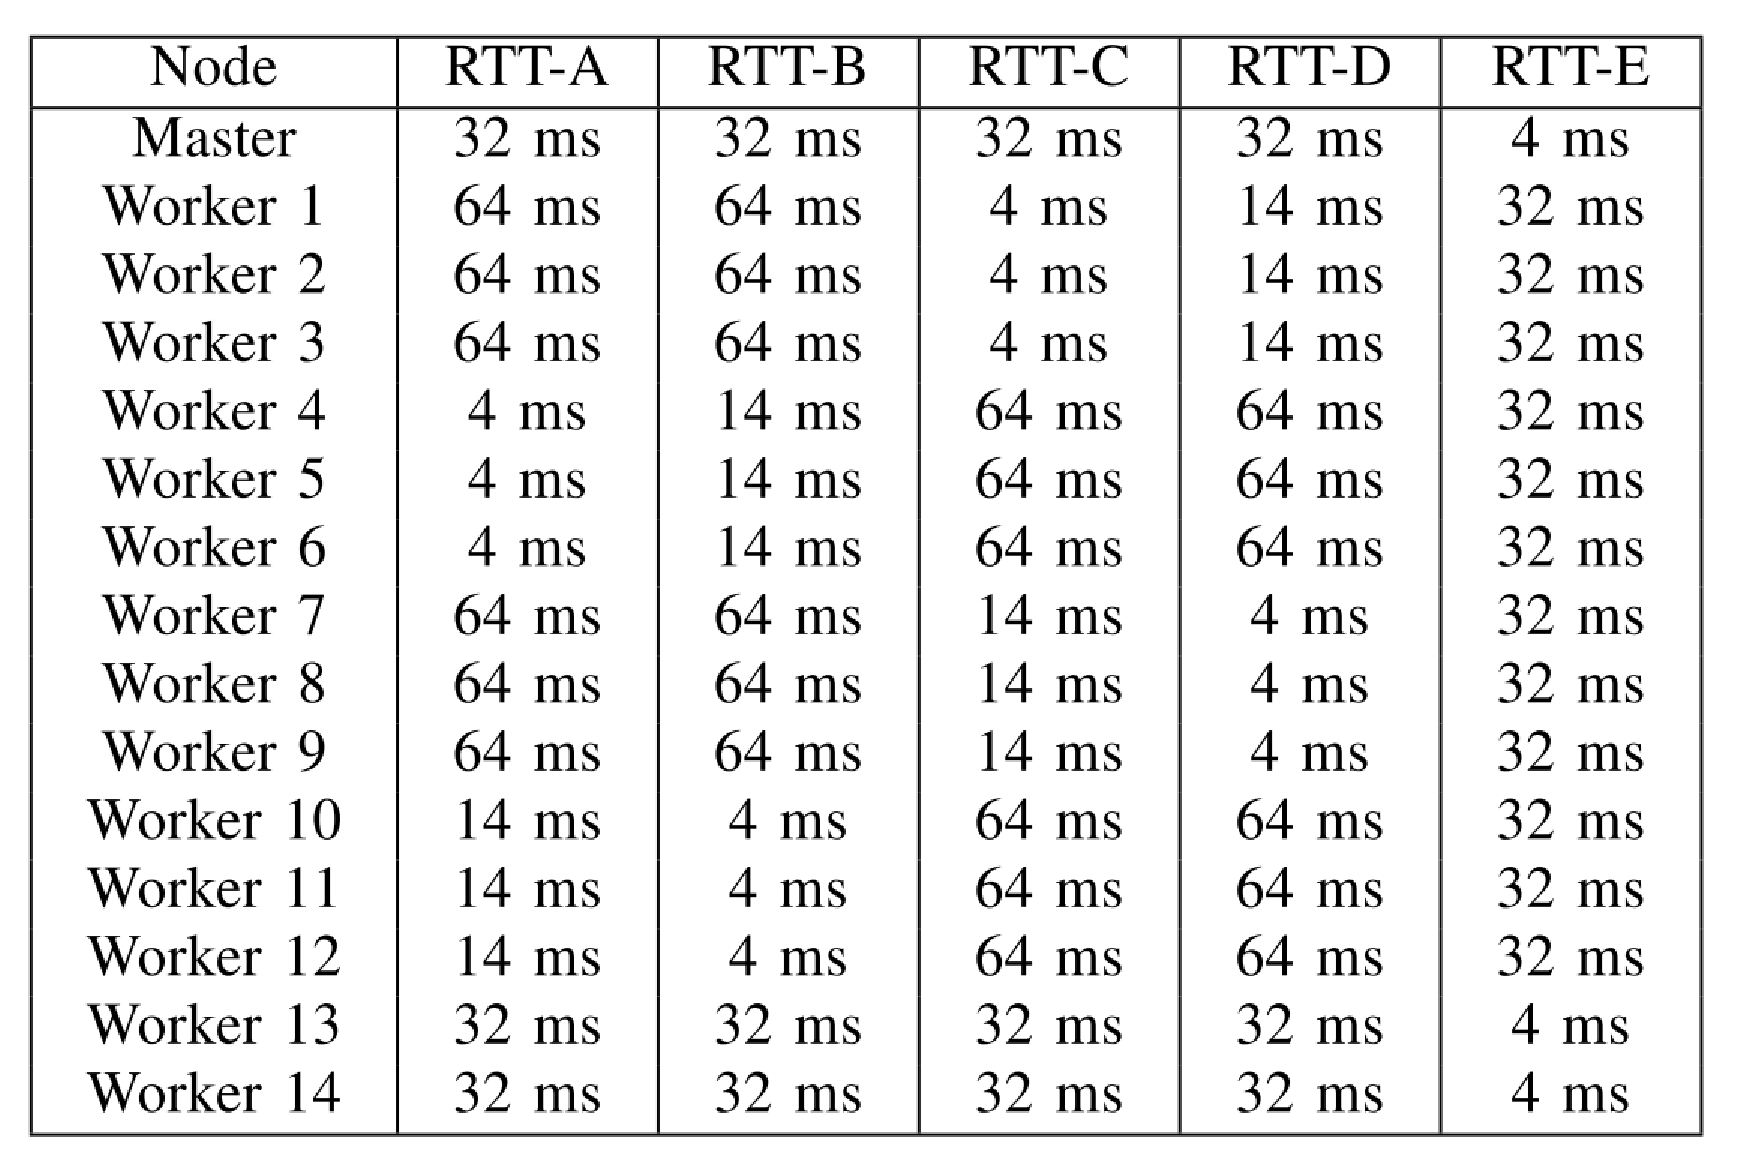
\includegraphics[width=\linewidth]{figures/mlcn-k8s-rtt.pdf}
  \caption{Location-based RTT values of \emph{nodes} in Fog Computing Infrastructure\cite{Santos2019}}
  \label{fig:k8s-rtt}
\end{figure}
\begin{figure}
  \centering
  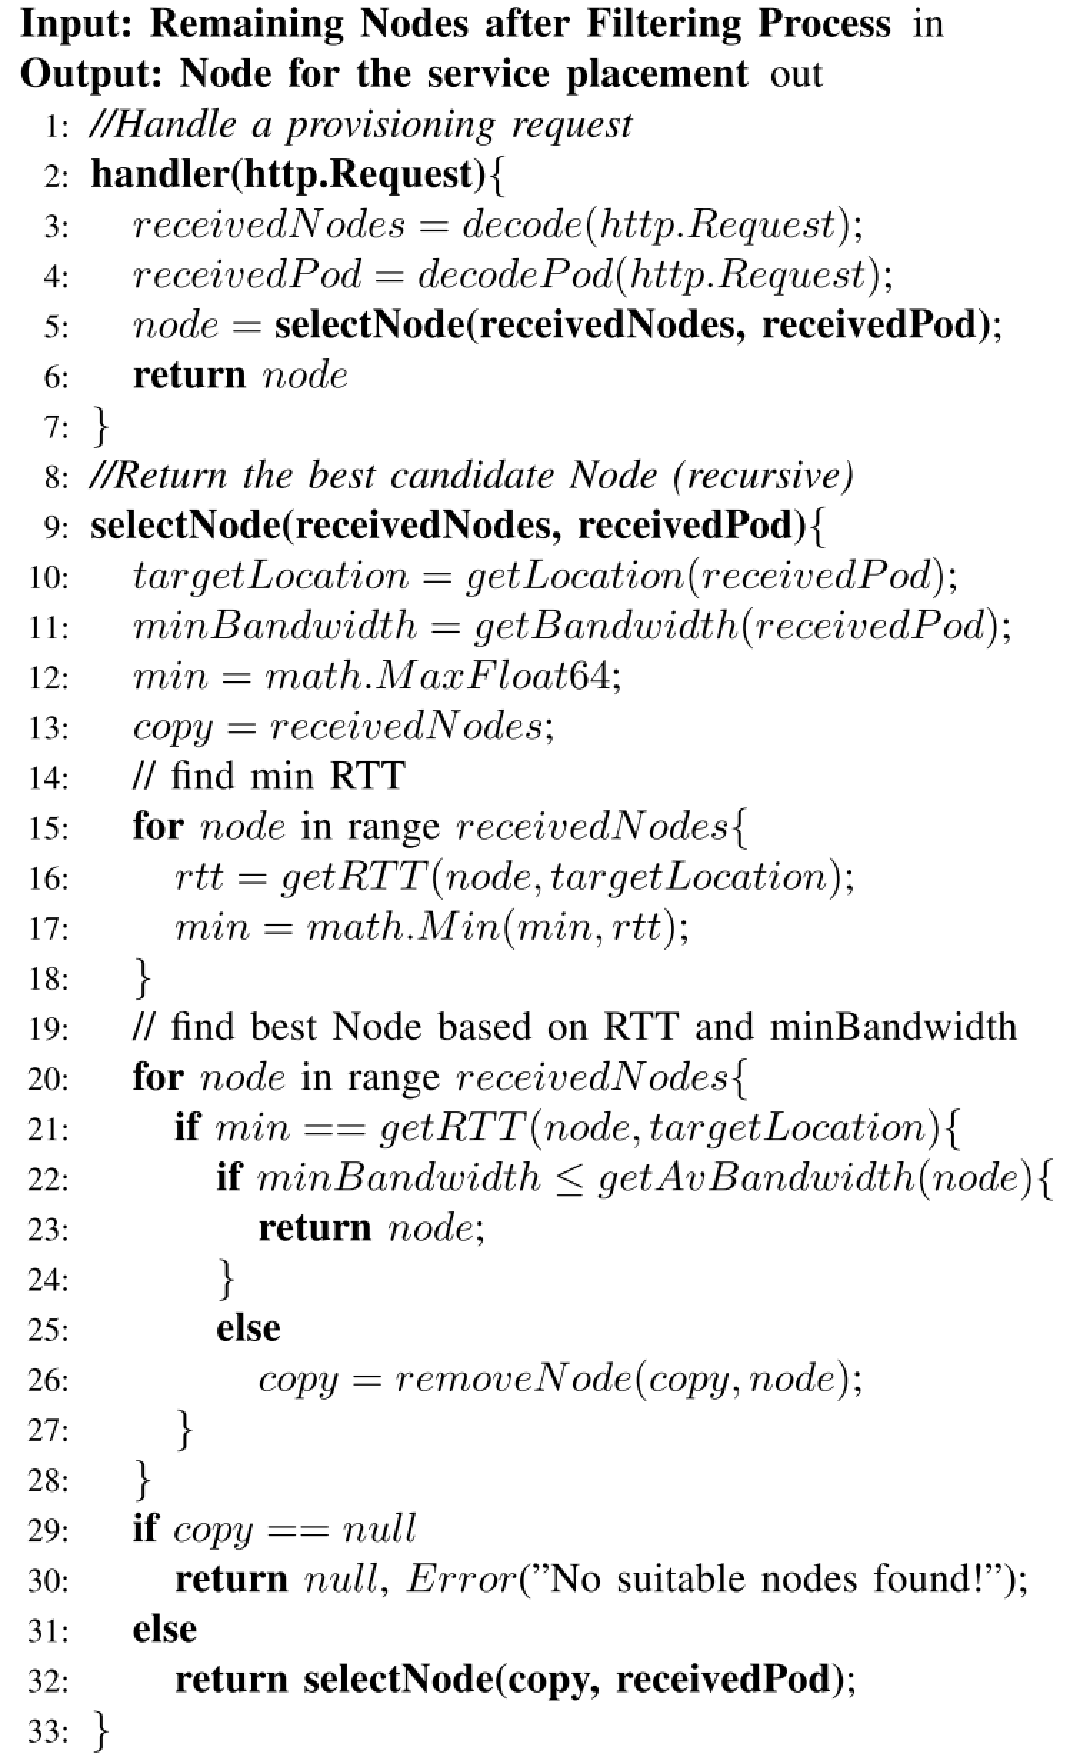
\includegraphics[width=\linewidth]{figures/mlcn-k8s-ns-algo.pdf}
  \caption{Network-Aware scheduling Algorithm\cite{Santos2019}}
  \label{fig:k8s-ns-algo}
\end{figure}
\begin{enumerate}
  \item \textbf{Random Scheduler:} This scheduler will get the input as a list of \emph{worker nodes} from \emph{Kibe-Scheduler} after applying \emph{filters/predicates} and output will be the randomly picked \emph{worker node} from the input list.
  \item \textbf{Network-Aware Scheduler:} This scheduler is based on the algorithm as shown in figure\ref{fig:k8s-ns-algo}. Based on the algorithm, input will be a list of \emph{worker nodes} from \emph{Kube-Scheduler} after applying \emph{filters/predicates}. After getting the deploy location from the \emph{pod} configuration file, this scheduler will make use of RTT labels to pick the best-fit \emph{worker node} having minimum RTT value\cite{Santos2019}. Apart from RTT based selection, this scheduler also look for the bandwidth label and check the \emph{pod} configuration file for bandwidth requirement. If no bandwidth requirement is specified then the scheduler consider 250KBit/s by default and returns the \emph{worker node} having minimum RTT and more bandwidth\cite{Santos2019}.
\end{enumerate}
\section{Performance Evaluation}
\label{sec:Performance_eval}
\begin{figure}
  \centering
  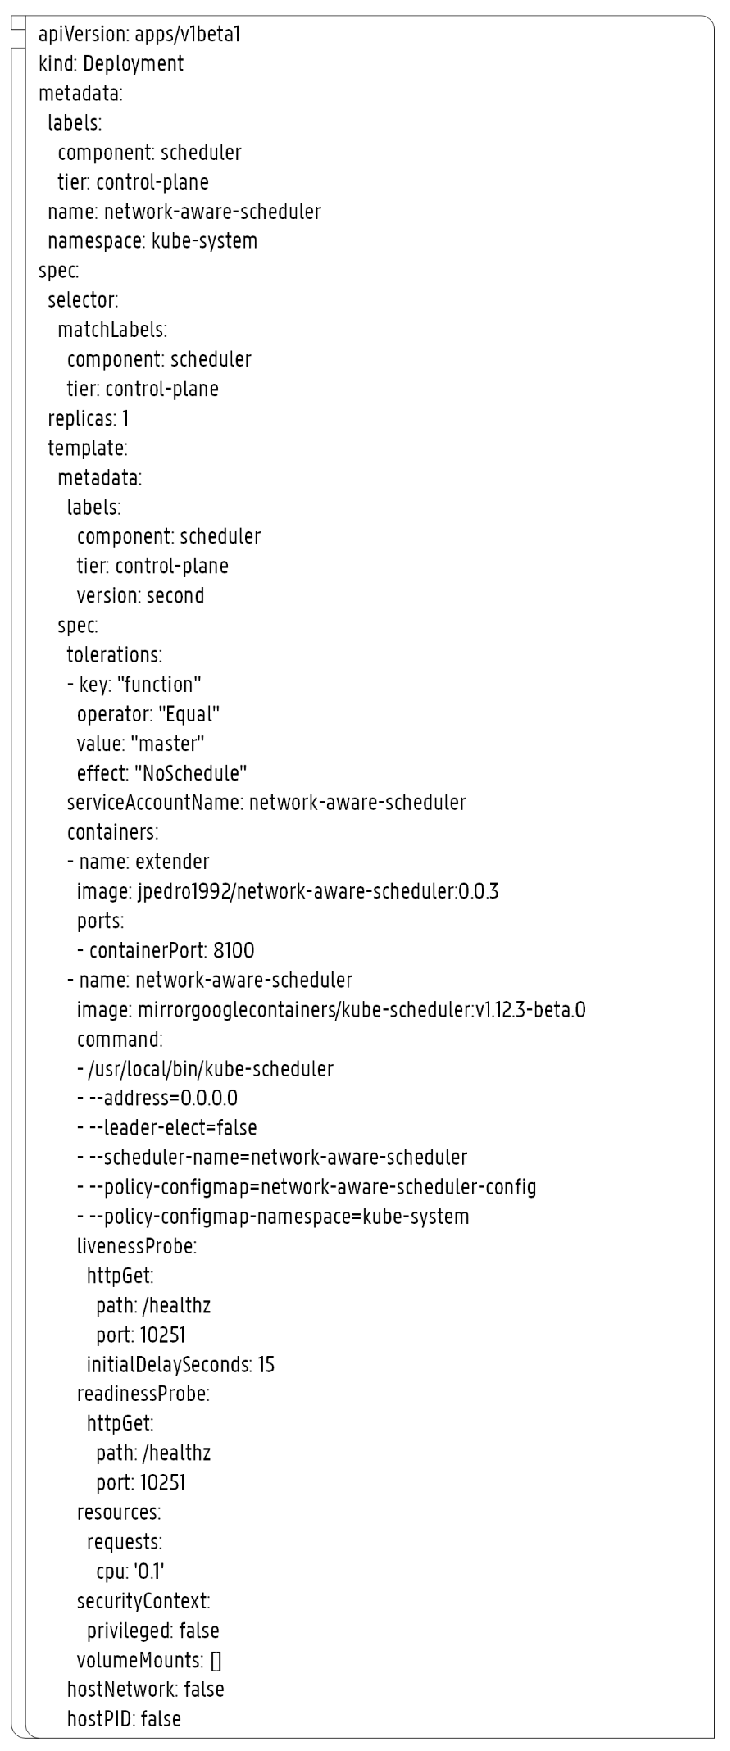
\includegraphics[width=75mm, height=20cm]{figures/mlcn-k8s-pod-config.pdf}
  \caption{\emph{Pod} Configuration for Scheduler\cite{Santos2019}}
  \label{fig:k8s-pod-config}
\end{figure}
In order to test the network-based resource provisioning for Fog Computing, Smart city scenario was considered \cite{Santos2019}. This scenario collects the air quality data of Antwerp city for organic compounds in the atmosphere \cite{Santos2019}.
\subsection{Expermentation Setup}
\label{sec:setup}
This smart city scenario was tested using the infrastructure as shown in figure\ref{fig:fog-k8s-infra}. This infrastructure was setup at IDLab, Belgium\cite{Santos2019}. The proposed network-based resource provisioning/network-aware scheduler was developed using Go and used as a \emph{pod} in Kubernetes cluster\cite{Santos2019}. Figure\ref{fig:k8s-pod-config} shows the \emph{pod} configuration that consists of two containers, the first container "extender" performs the network-aware resource scheduling operations whereas the second container "network-aware-scheduler" is the \emph{Kube-Scheduler} itself\cite{Santos2019}. Configuration can be seen in figure\ref{fig:k8s-sch-config}, where it can be seen that first \emph{Kube-scheduler} operations are performed afterward "extender" is called that performs the network-aware scheduling based on algorithm as shown in figure\ref{fig:k8s-ns-algo}. \par
\begin{figure}
  \centering
  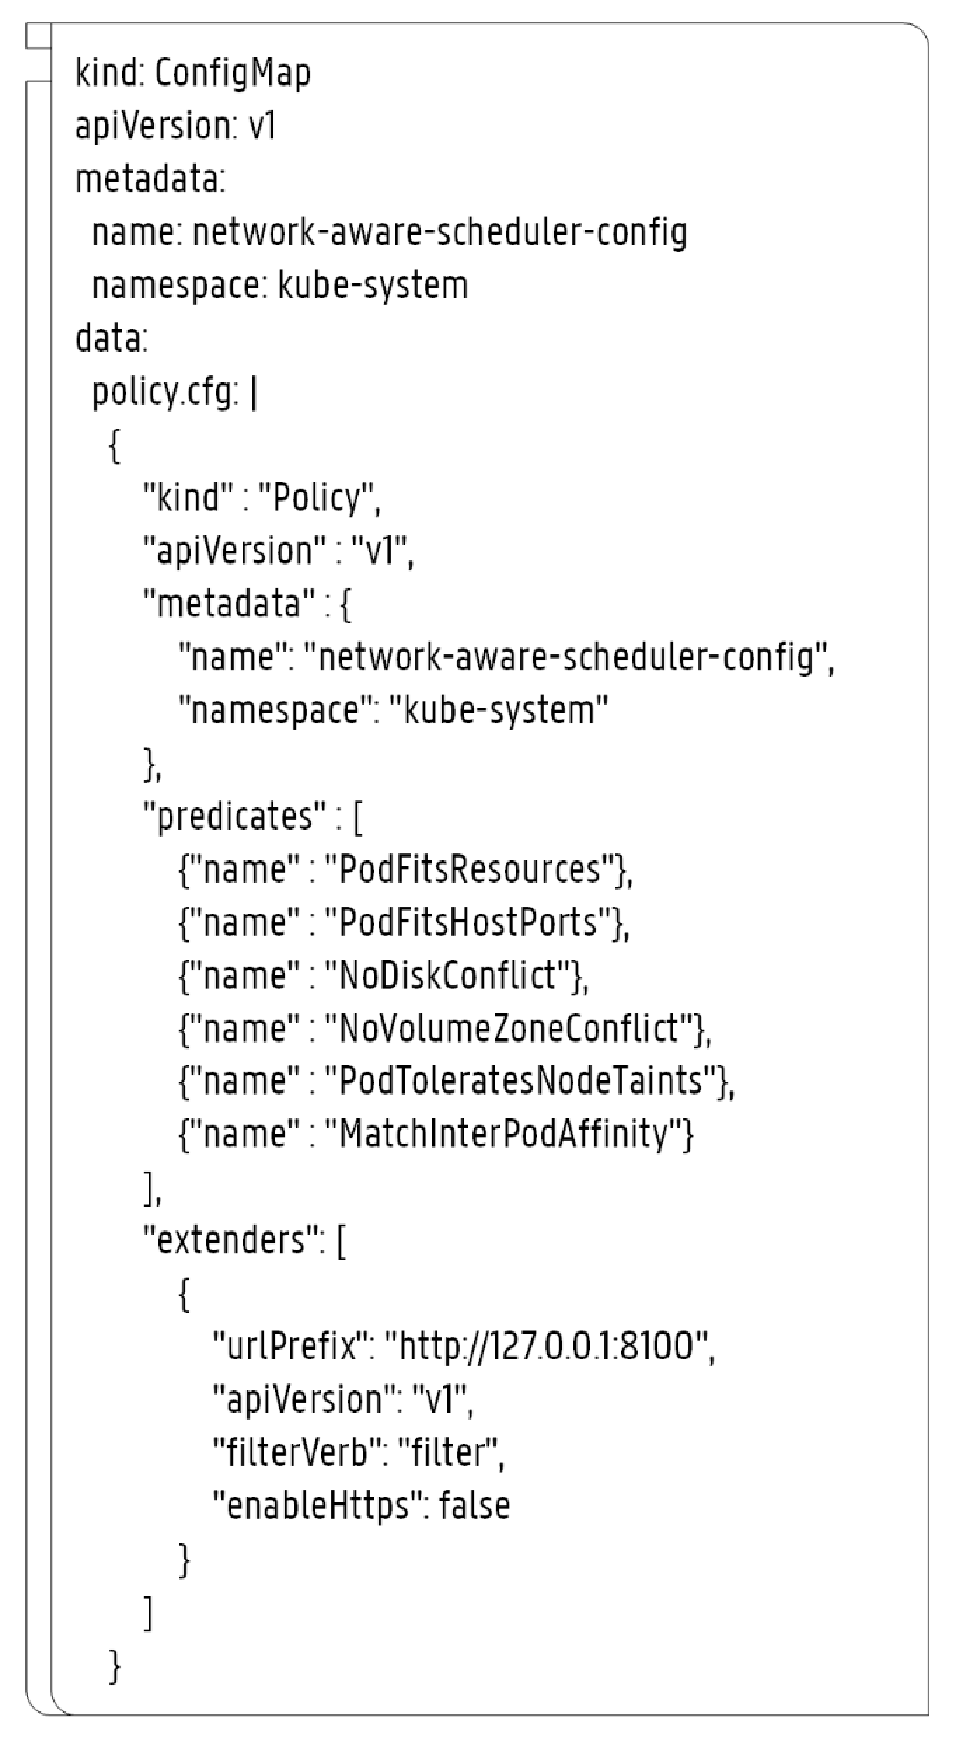
\includegraphics[width=\linewidth, height=8cm]{figures/mlcn-k8s-scheduler-config.pdf}
  \caption{\emph{Kube-Scheduler} Configuration\cite{Santos2019}}
  \label{fig:k8s-sch-config}
\end{figure}
\begin{figure*}
  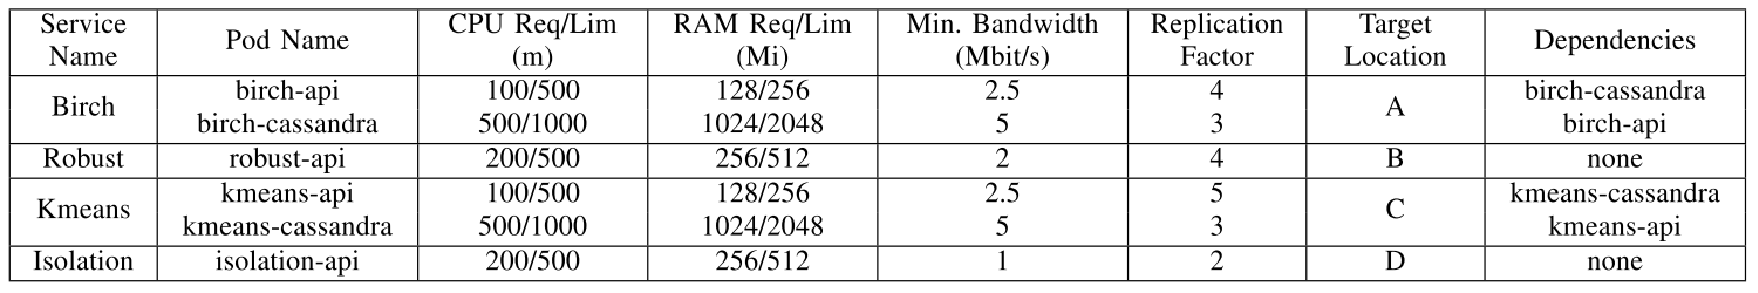
\includegraphics[width=\linewidth]{figures/mlcn-k8s-service-pods.pdf}
  \caption{Smart city deployed services\cite{Santos2019}}
  \label{fig:k8s-sch-config}
\end{figure*}
In the smart city scenario, many services were deployed as shown in figure\ref{fig:k8s-sch-config}. All the services were deployed either single or multiple \emph{pods}. Figure\ref{fig:k8s-sch-config} shows all the defined parameters in the configuration file against each \emph{pod}. The data collection of air quality was done through the algorithm and implemented as a container which is deployed as \emph{pod} namely "birch-api"\cite{Santos2019}. The \emph{pod} configuration of "birch-api" is similar to one shown in figure\ref{fig:k8s-pod-config}. Each \emph{pod} of the service  had some additional parameters in a \emph{pod} configration file such as "\emph{targetLocation}" that will define the deploy location in Fog Infrastructure as shown in figure\ref{fig:fog-k8s-infra}. Another parameter "\emph{bandwidthReq}" that defines the minimum required bandwidth for \emph{pod} deployment. Furthermore, in \emph{pod} configuration file, the \emph{affinity} parameter was set to \emph{podAntiAffinity} which limits the \emph{pods} of same service deploying on same the \emph{worker node}\cite{Santos2019}.
\begin{figure}
  \centering
  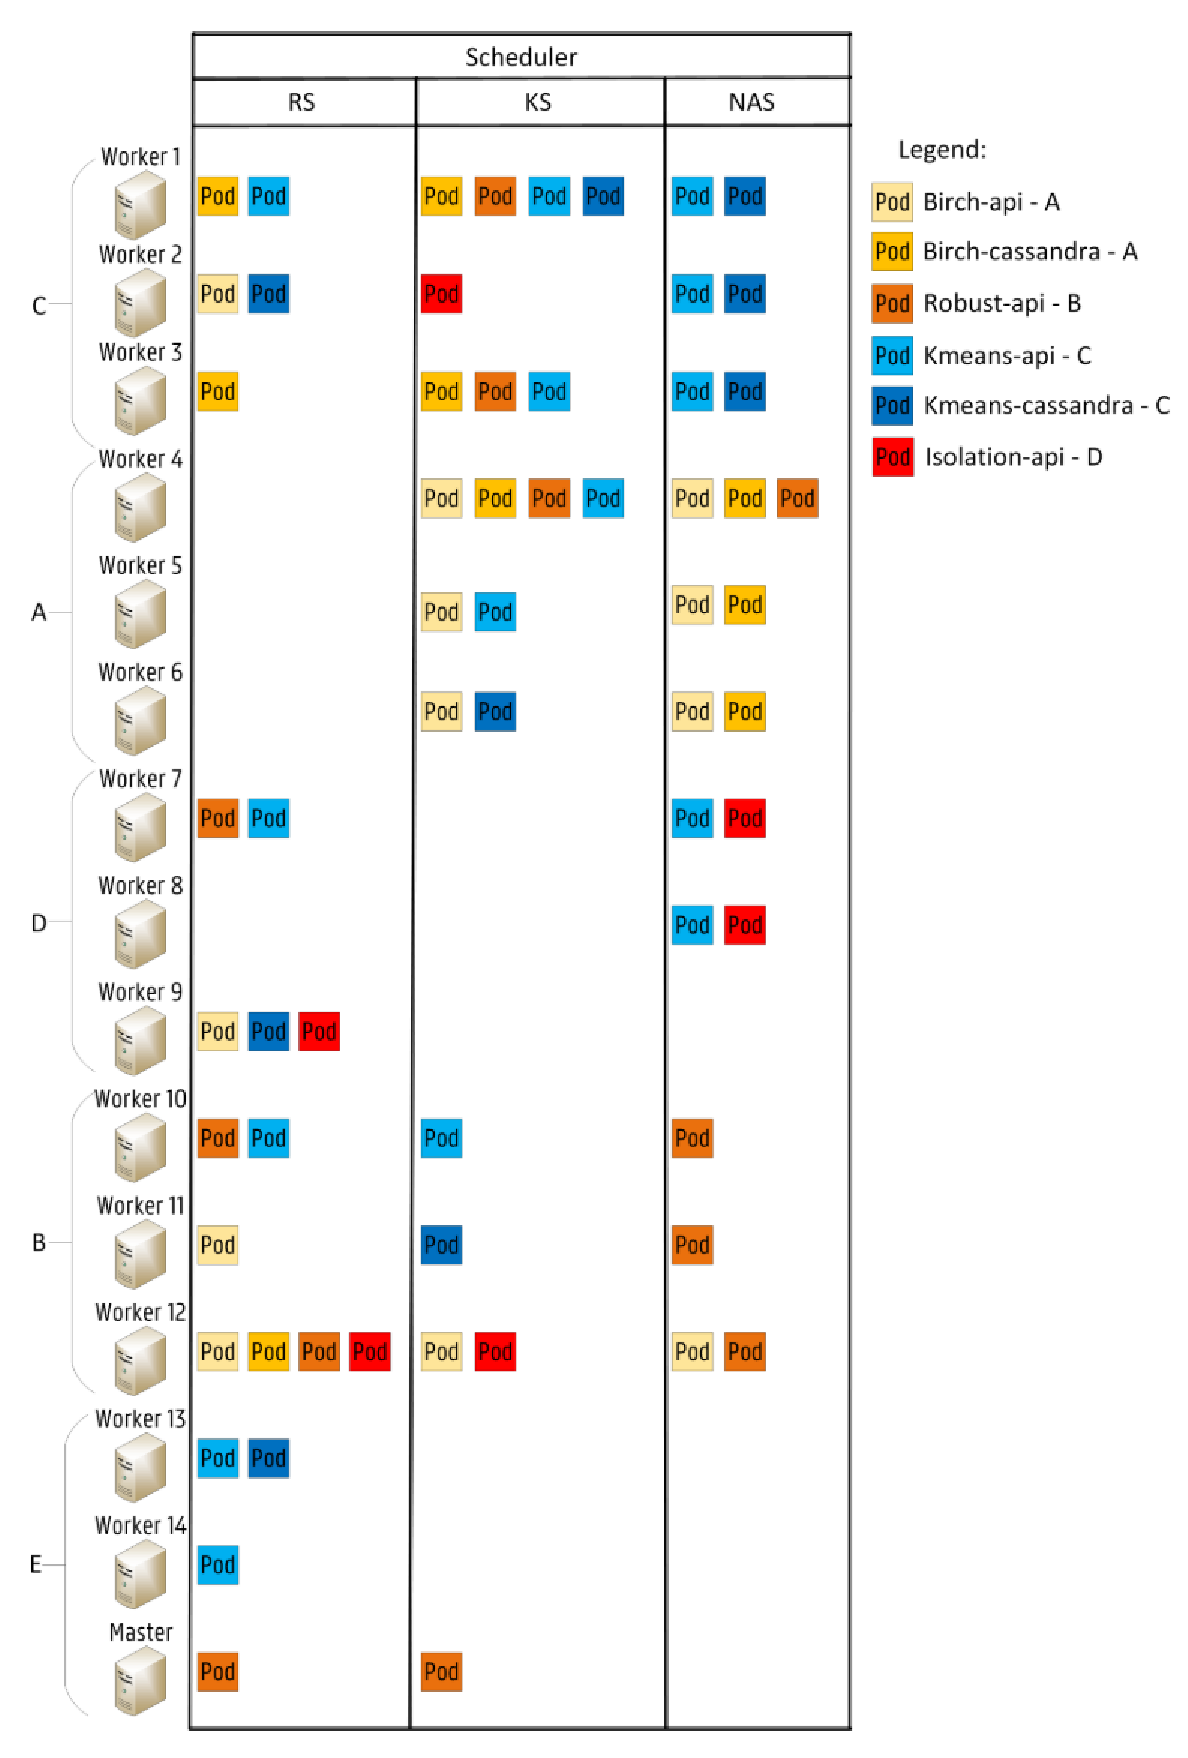
\includegraphics[width=\linewidth]{figures/mlcn-k8s-service-prov.pdf}
  \caption{Service deployment using different scheduling techniques\cite{Santos2019}}
  \label{fig:k8s-service}
\end{figure}
\begin{figure}
  \centering
  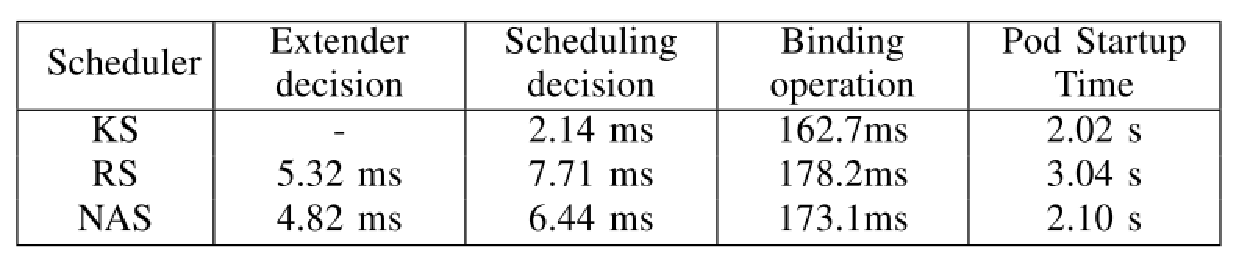
\includegraphics[width=\linewidth]{figures/mlcn-k8s-exec-time.pdf}
  \caption{Processing time of different scheduling techniques\cite{Santos2019}}
  \label{fig:k8s-exec-t}
\end{figure}
\begin{figure}
  \centering
  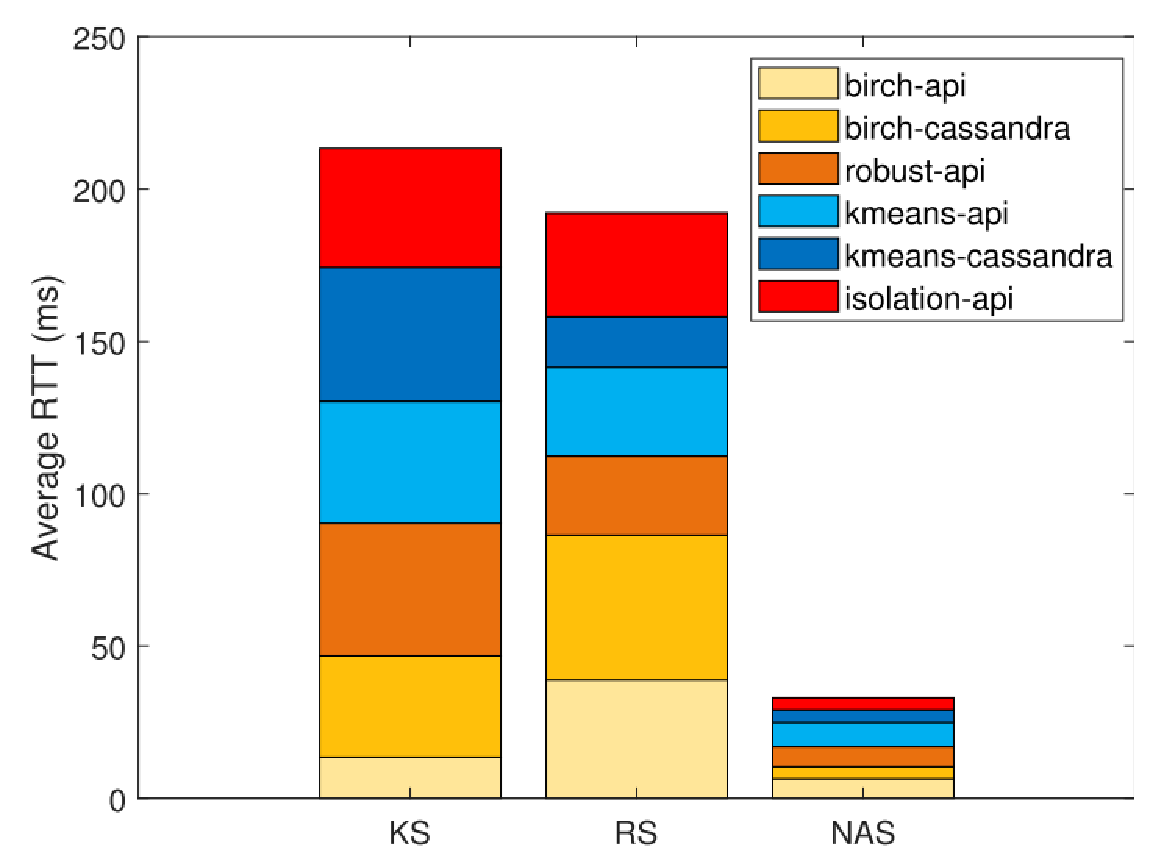
\includegraphics[width=\linewidth]{figures/mlcn-k8s-scheduler-compare.pdf}
  \caption{Average RTT of service deployment using different scheduling techniques\cite{Santos2019}}
  \label{fig:k8s-comapre-sc}
\end{figure}
\subsection{Analysis of Kubernetes Default and Network-based Resource Provisioning}
\label{sec:analysis}
In order to check the Performance of network-based resource provisioning scheduler, services in figure\ref{fig:k8s-sch-config} were deployed using default \emph{Kube-Scheduler(KS)}, Random Scheduler(RS), and Network-Aware Scheduler(NAS) as shown in figure\ref{fig:k8s-service}. It can be seen in figure\ref{fig:k8s-service} that both \emph{Kube-Scheduler} and Random Scheduler performs poorly by not taking the deploy location factor into account this leads to increased network latency\cite{Santos2019}. Taking an example of "\emph{Isolation-api}", whose desired deploying position was Location D, whereas it was not deployed properly by both \emph{Kube-Scheduler} and Random Scheduler\cite{Santos2019}. Figure\ref{fig:k8s-exec-t} shows the processing time of different schedulers for deploying \emph{pods}. \emph{Kube-Scheduler} on average takes 2.14ms for making scheduling decisions and in case of Random Scheduler and Network-aware Scheduler takes around 7.71ms and 6.44ms respectively\cite{Santos2019}. This added delay is due to an external process calls as discussed in section\ref{sec:k8s_ns}. After scheduling decision, for resource provisioning and starting \emph{pod} containers on \emph{worker node} time taken by \emph{Kube-Scheduler} and Network-Aware Scheduler was average 2 seconds whereas for Random schedulers it was 3 seconds\cite{Santos2019}. Further figure\ref{fig:k8s-service} shows that using \emph{Kube-Scheduler} and Random Scheduler overloads the \emph{worker node} in terms of bandwidth requirement as defined bandwidth per \emph{worker node} is 10Mbit/s\cite{Santos2019}. For example, \emph{Kube-Scheduler} deploys 4 \emph{pods} on \emph{worker node}1 and 4 exceeding the bandwidth of \emph{worker nodes} this leads to service interuption due to bandwidth\cite{Santos2019}. This issue was resolved when using Network-Aware Scheduler as it allows add minimum bandwidth requirement using "\emph{bandwidthReq}" in \emph{pod} configuration file. Figure\ref{fig:k8s-comapre-sc} shows the average RTT taken by different schedulers for \emph{pod} deployments. It shows thats Network-based resource scheduling/Network-Aware Scheduler outstands the \emph{Kube-Scheduler} and Random Scheduler by having very less RTT for each \emph{pod} deployment\cite{Santos2019}. For instance, average RTT for "\emph{Isolation-api}" is 4ms when deployed using Network-Aware Scheduler, and its very high for \emph{Kube-Scheduler} and Random Scheduler that is 39ms and 34ms respectively\cite{Santos2019}. Results show that by adding a few miliseconds for Network-Aware scheduling performance can be improved for service deployment in terms of network latency compare to \emph{Kube-Scheduler}\cite{Santos2019}.
\section{Comparison of Network-based Resource Provisioning Solutions}
\label{sec:related_work}
In this section, the Network-based resource provisioning technique is compared with the other solutions that allow resource provisioning in Fog Computing. This comparison is done based on the available orchestrator for fog computing and resource provisioning techniques.
\subsection{Orchestrator}
\label{sec:infra}
There are many orchestrators currently available, one such orchestrator is Fogernetes\cite{Wobker2018}. Fogernetes\cite{Wobker2018} platform is specially built for fog and edge applications and make use of heterogeneous devices. Fogernetes\cite{Wobker2018} has three layers namely cloud, fog, and edge. Similar to the Kubernetes-based solution\cite{Santos2019}, it also uses the labeling system to identify the layer, location, performance, and connectivity\cite{Wobker2018}. Fogernetes\cite{Wobker2018} platform was tested against surveillance application, that collects data from multiple cameras. Kubernetes was used for the implementation of Fogernetes\cite{Wobker2018}. Three Kubernetes nodes were used one for each layer of Fogernetes\cite{Wobker2018}. Out of three nodes, 2 nodes were servers that were labeled as cloud and fog and the third node was Rasberry Pi labeled as edge. Camera works on edge layer that transfers the data to fog layer for processing and afterward it is stored in cloud layer. Monitoring of these layers can be done through the  Kubernetes Dashboard or external Dashboard Grafana. Compare to the solution of base-paper\cite{Santos2019}, Fogernetes\cite{Wobker2018} tested the Fog Computing application in true manner, by deploying services on heterogeneous devices. \par
Another orchestrator is presented in \cite{Reale} build on top of Docker Swarm. This orchestrator considers the dynamic nature of the network and automates the distribution of the services across the nodes in the Fog Computing environment\cite{Reale}. This solution is based on peer-to-peer collaborative computation network that tries to map available resources, plans the deployment, move the services across the nodes, and monitoring of overall infrastructure\cite{Reale}. In base-paper solution\cite{Santos2019} Kubernetes was used as the infrastructure whereas in \cite{Reale} Docker Swarm was used. One key feature of using a solution\cite{Reale} is that it allows the \emph{live migration} of service when the node is exhausted in terms of computation, network latency. This feature is currently lagging in base-paper solution\cite{Santos2019}.
\subsection{Resource Provisioning Techniques}
There are many resource provisioning techniques/schedulers currently available for Kubernetes-based Fog Computing infrastructure. One such scheduler is presented in \cite{Haja2019}, that deploys the services taking network delay into account. This scheduler\cite{Haja2019} has the following features: checks for node latency periodically and updates the node label with the latest latency value, supports \emph{pod} re-scheduling in-case of network delays. This Scheduler\cite{Haja2019} selects the \emph{worker node} using the "greedy heuristic algorithm". This scheduler\cite{Haja2019} performs better than Network-Aware Scheduler\cite{Santos2019} in two ways: first, continuously updating the latency that helps in the efficient deployment of \emph{pods} and second the re-scheduling of the \emph{pod} from one \emph{worker node} to other in terms of \emph{worker node} failure and network delay. These two features are currently not present in Network-Aware Scheduler. \par
DYSCO\cite{Mittermeier2018} is yet another scheduler for Kubernetes resource provisioning. DYSCO takes following contextual elements to for service deployment across nodes\cite{Mittermeier2018}: "Node Name", "Compute Domain"(cloud, fog, edge), "Location", "Computing Power", "Processor Architecture"(amd64, arm, etc.), "Memory" and "Network Connectivity"(GSM, 3G, LTE, DSL, etc.). DYSCO is also fault-tolerant in case of node failure and network breakdown\cite{Mittermeier2018}. Compare to Network-Aware Scheduler\cite{Santos2019}, DYSCO has additional filters such as processor type and network-connectivity type but it does not tackle the latency and bandwidth issues. \par
The Scheduler proposed in \cite{8903766} works alongside the default \emph{Kube-Scheduler} as an external asynchronous module. \emph{Kube-Scheduler} performs the operations in two steps: \emph{node filtering} and \emph{node scoring} whereas This Scheduler\cite{8903766} performs the operation in a single step and works as follows: continuously collects the real-time data such as CPU usage, available Memory, latency, packet loss, etc.  for all \emph{worker nodes}. Afterward the scheduling is applied for \emph{pod} deployment. Scheduling algorithm consists of the following steps: the list of pending \emph{pods} to be deployed. Re-arrange them in descending order meaning \emph{pod} with high resource requirement comes first. As mentioned in \cite{8903766}, "Knapsack problem greedy approach" was used which is an optimization technique that will arrange \emph{worker nodes} in a list based on best-fit criteria of \emph{pod} resource requirement fulfillment. The next step, each node is checked for Liveness(status of node: busy, ready, etc.), available CPU, and available Memory\cite{8903766}. Lastly, node scoring is done based on the real-time resource utilization data from the \emph{worker node}. The \emph{worker node} with less resource utilization value is considered the best candidate\cite{8903766}. Compare to Network-Aware Scheduler\cite{Santos2019}, this scheduler\cite{8903766} is a complete scheduler itself, whereas Network-aware Scheduler\cite{Santos2019} is an extension of default \emph{Kube-Scheduler}. The proposed scheduler in \cite{8903766} is more complex but uses the optimization techniques that result in efficient scheduling.
\section{Conclusion}
\label{sec:concl}
The aim of Fog Computing is to bring computational resources nearer to the end-user with minimum network utilization. Fog Computing enabled many IoT applications but there is no proper management and orchestration. This seminar paper presented the Kubernetes-based solution for IoT applications. All the applications are deployed as \emph{pod} consist of single or multiple Docker containers. Default Kubernetes scheduler does not consider the network utilization while deploying the \emph{pods} which goes against the Fog Computing. In order to cater the network utilization, this seminar paper also discussed about the new scheduling technique Network-Aware Scheduler that works along with the default scheduler and allows the \emph{pod} deployment based on network parameters such as RTT, latency, and bandwidth. The results mentioned in this seminar paper shows that the performance of Network-Aware Scheduler is far better compared to the default Kubernetes scheduler.
\section{Further Research Topics}
\label{sec:research}
Extend the Network-Aware Scheduler to re-schedule the \emph{pod} in case of node failure and network breakdown more efficiently. Adding more networking filters such as selecting connection types such as LAN, 3G, LTE, fiber, etc.
